\documentclass[]{article}
\usepackage{fullpage}
\usepackage{lastpage}
\usepackage[top=1in,bottom=1in,margin=1in]{geometry}
\usepackage{supertabular}
\usepackage{graphicx,tikz}	
%\usepackage{tkz-euclide}
%\usetkzobj{all}
\usetikzlibrary{calc}
\usepackage{array,multicol}
\usepackage{amsmath,amssymb}
\usepackage{enumitem}

\usepackage{fancyhdr}
\pagestyle{fancy}

\addtolength{\topmargin}{-0.25in}

\newcommand{\vect}[1]{\mathbf{#1}}
\DeclareMathOperator{\proj}{proj}

\fancypagestyle{plain}{
	\addtolength{\headheight}{0.485in}
	\rhead{\bf MATH 2574 (Calculus III) \\
		%\vspace{0.5pc}
		Wed 8 Mar 2017 \\}
	\rfoot{\footnotesize $\;$Quiz 6IC, p. \thepage\ (of \pageref{LastPage})
	}
\renewcommand{\headrulewidth}{0pt}
}
\fancyhf{}
\renewcommand{\headrulewidth}{0pt}
\rfoot{\footnotesize Quiz 6IC, p. \thepage\ (of \pageref{LastPage})$\;$}

\title{\vspace{-3.5pc} 
	\flushleft \bf \Large In-Class Quiz 6: Double integrals in polar coordinates \\ (\S 13.3)}
\date{}

% % % % %
\begin{document}
\maketitle

\vspace{-3pc}
\noindent{\bf Directions:} This quiz is due at the end of lecture.  

\noindent\hrulefill

\begin{enumerate}

% % %
\item %{\bf \S13.3 \#20}
Find the volume of the solid bounded by the paraboloids $z=2x^2+y^2$ and $z=27-x^2-2y^2$ (see figure).

\begin{center}
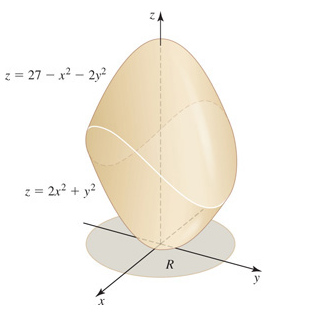
\includegraphics{13-3no20}
\end{center}

%\item %{\bf 13.3 \#22}
%Find the volume of the solid bounded by the paraboloid $z=8-x^2-3y^2$ and the hyperbolic para

% % % % %
\end{enumerate}
\end{document}